\chapter{Arquitetura Estabelecida}
\label{chap:Arquitetura}
	
	Nesta seção serão abordados tópicos ....

	TO DO.

	\section{Componentes da Arquitetura}
	\label{sec:Arquitetura_Componentes}

		Utilizou-se de 4 componentes para montar a infraestrutura necessária para o projeto. Cada uma com um papel e serviço específico. Além disso, metade dos componentes são máquina virtuais, instânciadas pelo software \emph{VMware}. A seguir, são elencados os componentes e suas respectivas caracteristicas:

		\begin{itemize}
			\item \textbf{Cliente Comum} - IP: \emph{192.168.0.12} - .

			- Características:
	
			\item \textbf{Cliente Malicioso} - IP: \emph{192.168.0.13} - .

			- Características:
	
			\item \textbf{Servidor IPS/IDS} - IP: \emph{192.168.0.42} - .

			- Características:
	
			\item \textbf{Servidor WEB} - IP: \emph{192.168.0.17} - .	

			- Características:
	
		\end{itemize}


	\section{Esquema da Infraestrutura}
	\label{sec:Arquitetura_Esquema_Infra}

		A figura \ref{fig:arquitetura} encontra-se a representação lógica da estrutura de redes estabalecida para este projeto.

		\begin{figure}[h]
			\centering
			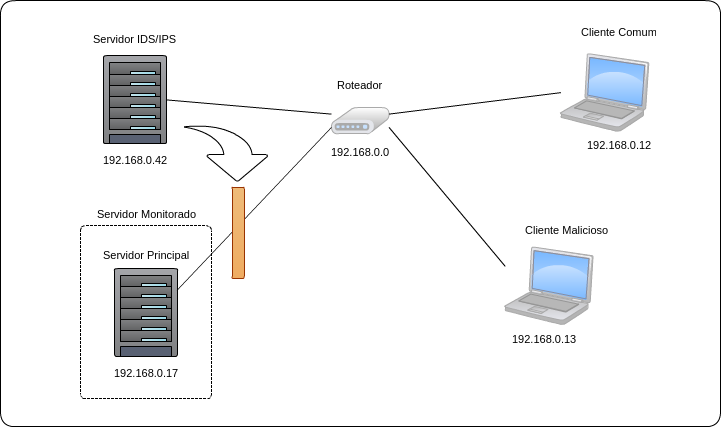
\includegraphics[scale=0.6]{arquitetura}
			\caption{Arquitetura estabelecida para o Projeto.}
			\label{fig:arquitetura}
		\end{figure}

	\section{Limitações}
	\label{sec:Arquitetura_Limitacoes}

		TO DO.

		